\chapter{Descending the Abyss}

\section{The Abyss}
In the middle of Orth lies the legendary abyss. It is a circular chasm that is 1 km across. It is a source of great pride and challenge, as well as worship for many of its citizens. The Abyss is fraught with dangers and is very difficult to navigate. Maps are spotty at best, and information is scarce. Most knowledge is shared from mouth to mouth. 

\begin{center}
\begin{tabular}{c}
\adjustbox{trim=0 0 0 0,clip}{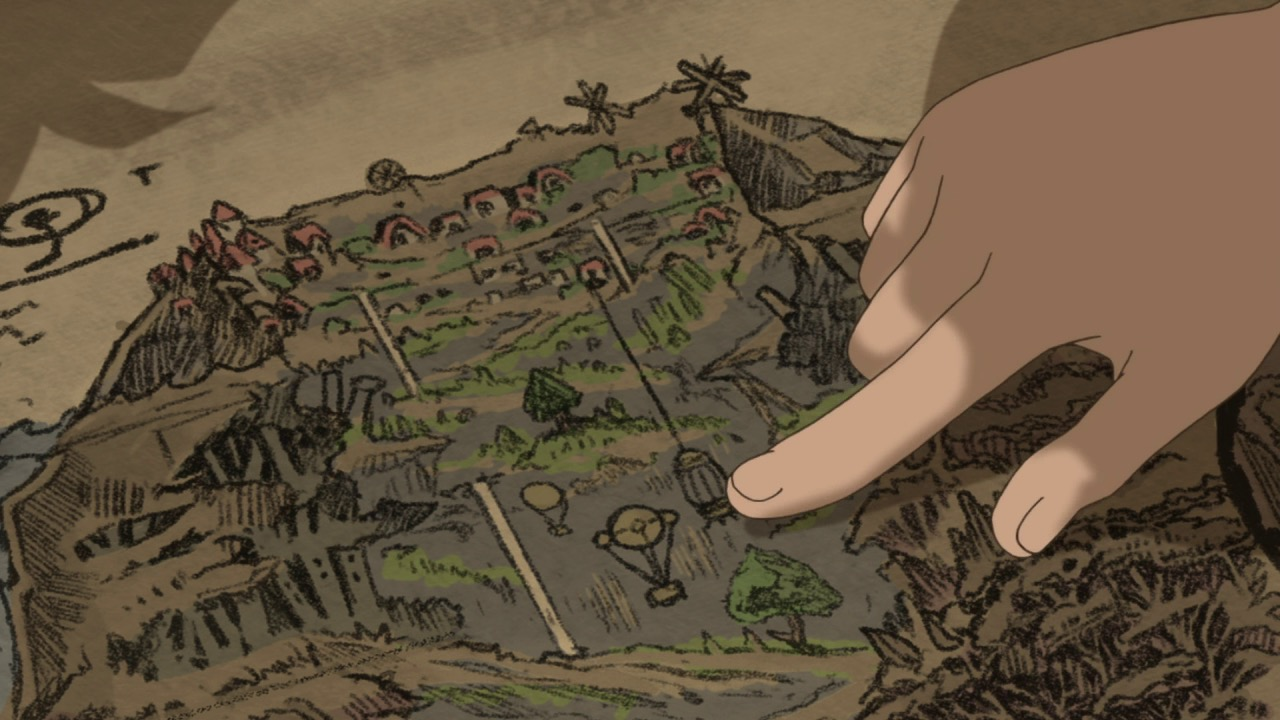
\includegraphics[width=8cm]{img/delvers/2.jpg}} \\
 \end{tabular}
\captionof{figure}{ Illustration of the village of Orth at the top, at the edge of the abyss. A delver pointing to its lower parts.}
\end{center}

\begin{table*}[t]
\header{Layers of the Abyss}
\centering
    \begin{dndtable}[clrX]
    \textbf{Layer} & \textbf{Name} & \textbf{Deepest (m)} & \textbf{Description}   \\
    Surface & Town of Orth                     & $0$     &                      \\
            1st & Edge of the Abyss                    & $1350$     &                      \\
            2nd & Forest of Temptation                 & $2600$     &                   \\
            3rd & Great Fault                          & $7000$     &                   \\
            4th & The Goblet of Giants                 & $12000$    &                   \\
            5th & Sea of Corpses                       & $13000$    &                  \\
            6th & The Capital of the Unreturned        & $15500$    &                  \\
            7th & The Final Maelstrom                  & ?            &                  \\
            8th &The Deepest Point                     & $>20000$   &                                \\
  \end{dndtable}
  \caption{Layers of the Abyss}
\end{table*}

\section{Dungeoneering}

Makes sense to tell the DM that any dungeon they can find would fit the abyss. A giant mushroom, a dungeon in an upside down windmill, underwater dungeon exploration. What is on the edge of the abyss's many layers? Sprinkle many different monsters. Take inspiration from here!

\section{Creatures of the Abyss}

Delvers diving into the abyss find themselves in a totally different ecosystem compared to the surface world. However, they will also discover themselves no longer on the top of the food chain. Delvers who have encountered creatures have categorized them depending on their danger level. The following table describes their levels. 

\header{Creature Classes}\label{tab:CreatureClasses}
\begin{dndtable}[lXc]
    \textbf{Class}  & \textbf{Rating} & \textbf{D\&D CR} \\
    Harmless    & \FiveStarOpen & 0\\
    Minor   & \FiveStar & 1\\
    Caution & \FiveStar \FiveStar & 2\\
    Serious & \FiveStar \FiveStar \FiveStar & 3-5\\
    Lethal  & \FiveStar \FiveStar \FiveStar \FiveStar & 6-9\\
    Irrational  & \FiveStar \FiveStar \FiveStar \FiveStar \FiveStar & 10-12\\
    Extraordinary   & \FiveStar \FiveStar \FiveStar \FiveStar \FiveStar \FiveStar & 13-15\\
    Unprecedented   & \FiveStar \FiveStar \FiveStar \FiveStar \FiveStar \FiveStar \FiveStar & 16+\\
\end{dndtable}

%\header{Creature Illustration}
%\begin{center}
%\begin{tabular}{c}
%\adjustbox{trim=0 0 0 %0,clip}{\includegraphics[width=8cm]{img/descending/151169500795%197.jpg}} \\
% \end{tabular}
%\captionof{figure}{ Drawing illustrations of creatures from the %lower depths of the abyss. Drawn by the white whistle, Lyza the %Annihilator. }
%\end{center}

Not only will delvers meet monstrous creatures, they will also find themselves in conflict with other delvers from foreign countries, looking to cash in on the abyss's treasures. These are considered hostile and should be disposed off. 

\subsection{Monster Manual \& Other Resources}
The opinion of the author is that the monster manual should be used sparingly, if ever. The argument is that this is a world that relies on exploration, as such, players need to feel a sense of wonder, awe, and dread, whenever they observe new settings and creatures. To achieve this effect, consider using the monster resources found at the \textbf{Monster A Day subreddit r/monsteraday/}\footnote{https://www.reddit.com/r/monsteraday/}. Each creature is descripted using 5 edition D\&D stat blocks with art work.

Choose creatures that fit the theme of each layer. When describing an encounter's difficulty, describe its visible features, and if applicable, allow players to consult their lexicon on creatures of the abyss. Use the creature class naming scheme during play to make players uneasy\ref{tab:CreatureClasses}.

\section{Artifacts}
Artifacts or relics are classified and cataloged according to their power. All artifacts have limited number of uses, often indicated by the strange writings on them. The most powerful artifacts that a white whistle can use are second grade artifacts. Greater artifacts are considered very important to national security and can be found deep within the abyss. 

\begin{quotebox}
	The discovery of a Greater Artifact is a huge ordeal. Experts and White whistles are tasked with their retrieval. These trips are perilous, as such, often come at the great cost of many lives. Greater artifacts are not cataloged, or only partially, to keep them secret from other nations, thus keeping an edge in the power struggle.
\end{quotebox}

\header{Artifact Classes}
\begin{dndtable}[lX]
  \textbf{Classes} & \textbf{Description} \\
  Special Grade Artifact            &  \\
  First Grade Artifact            &  \\
  Second Grade Artifact            &  \\
  Third Grade Artifact            &  \\
  Fourth Grade Artifact            &  \\
\end{dndtable}

\newpage

\begin{figure}[ht]
  \afterpage{%
    \noindent
    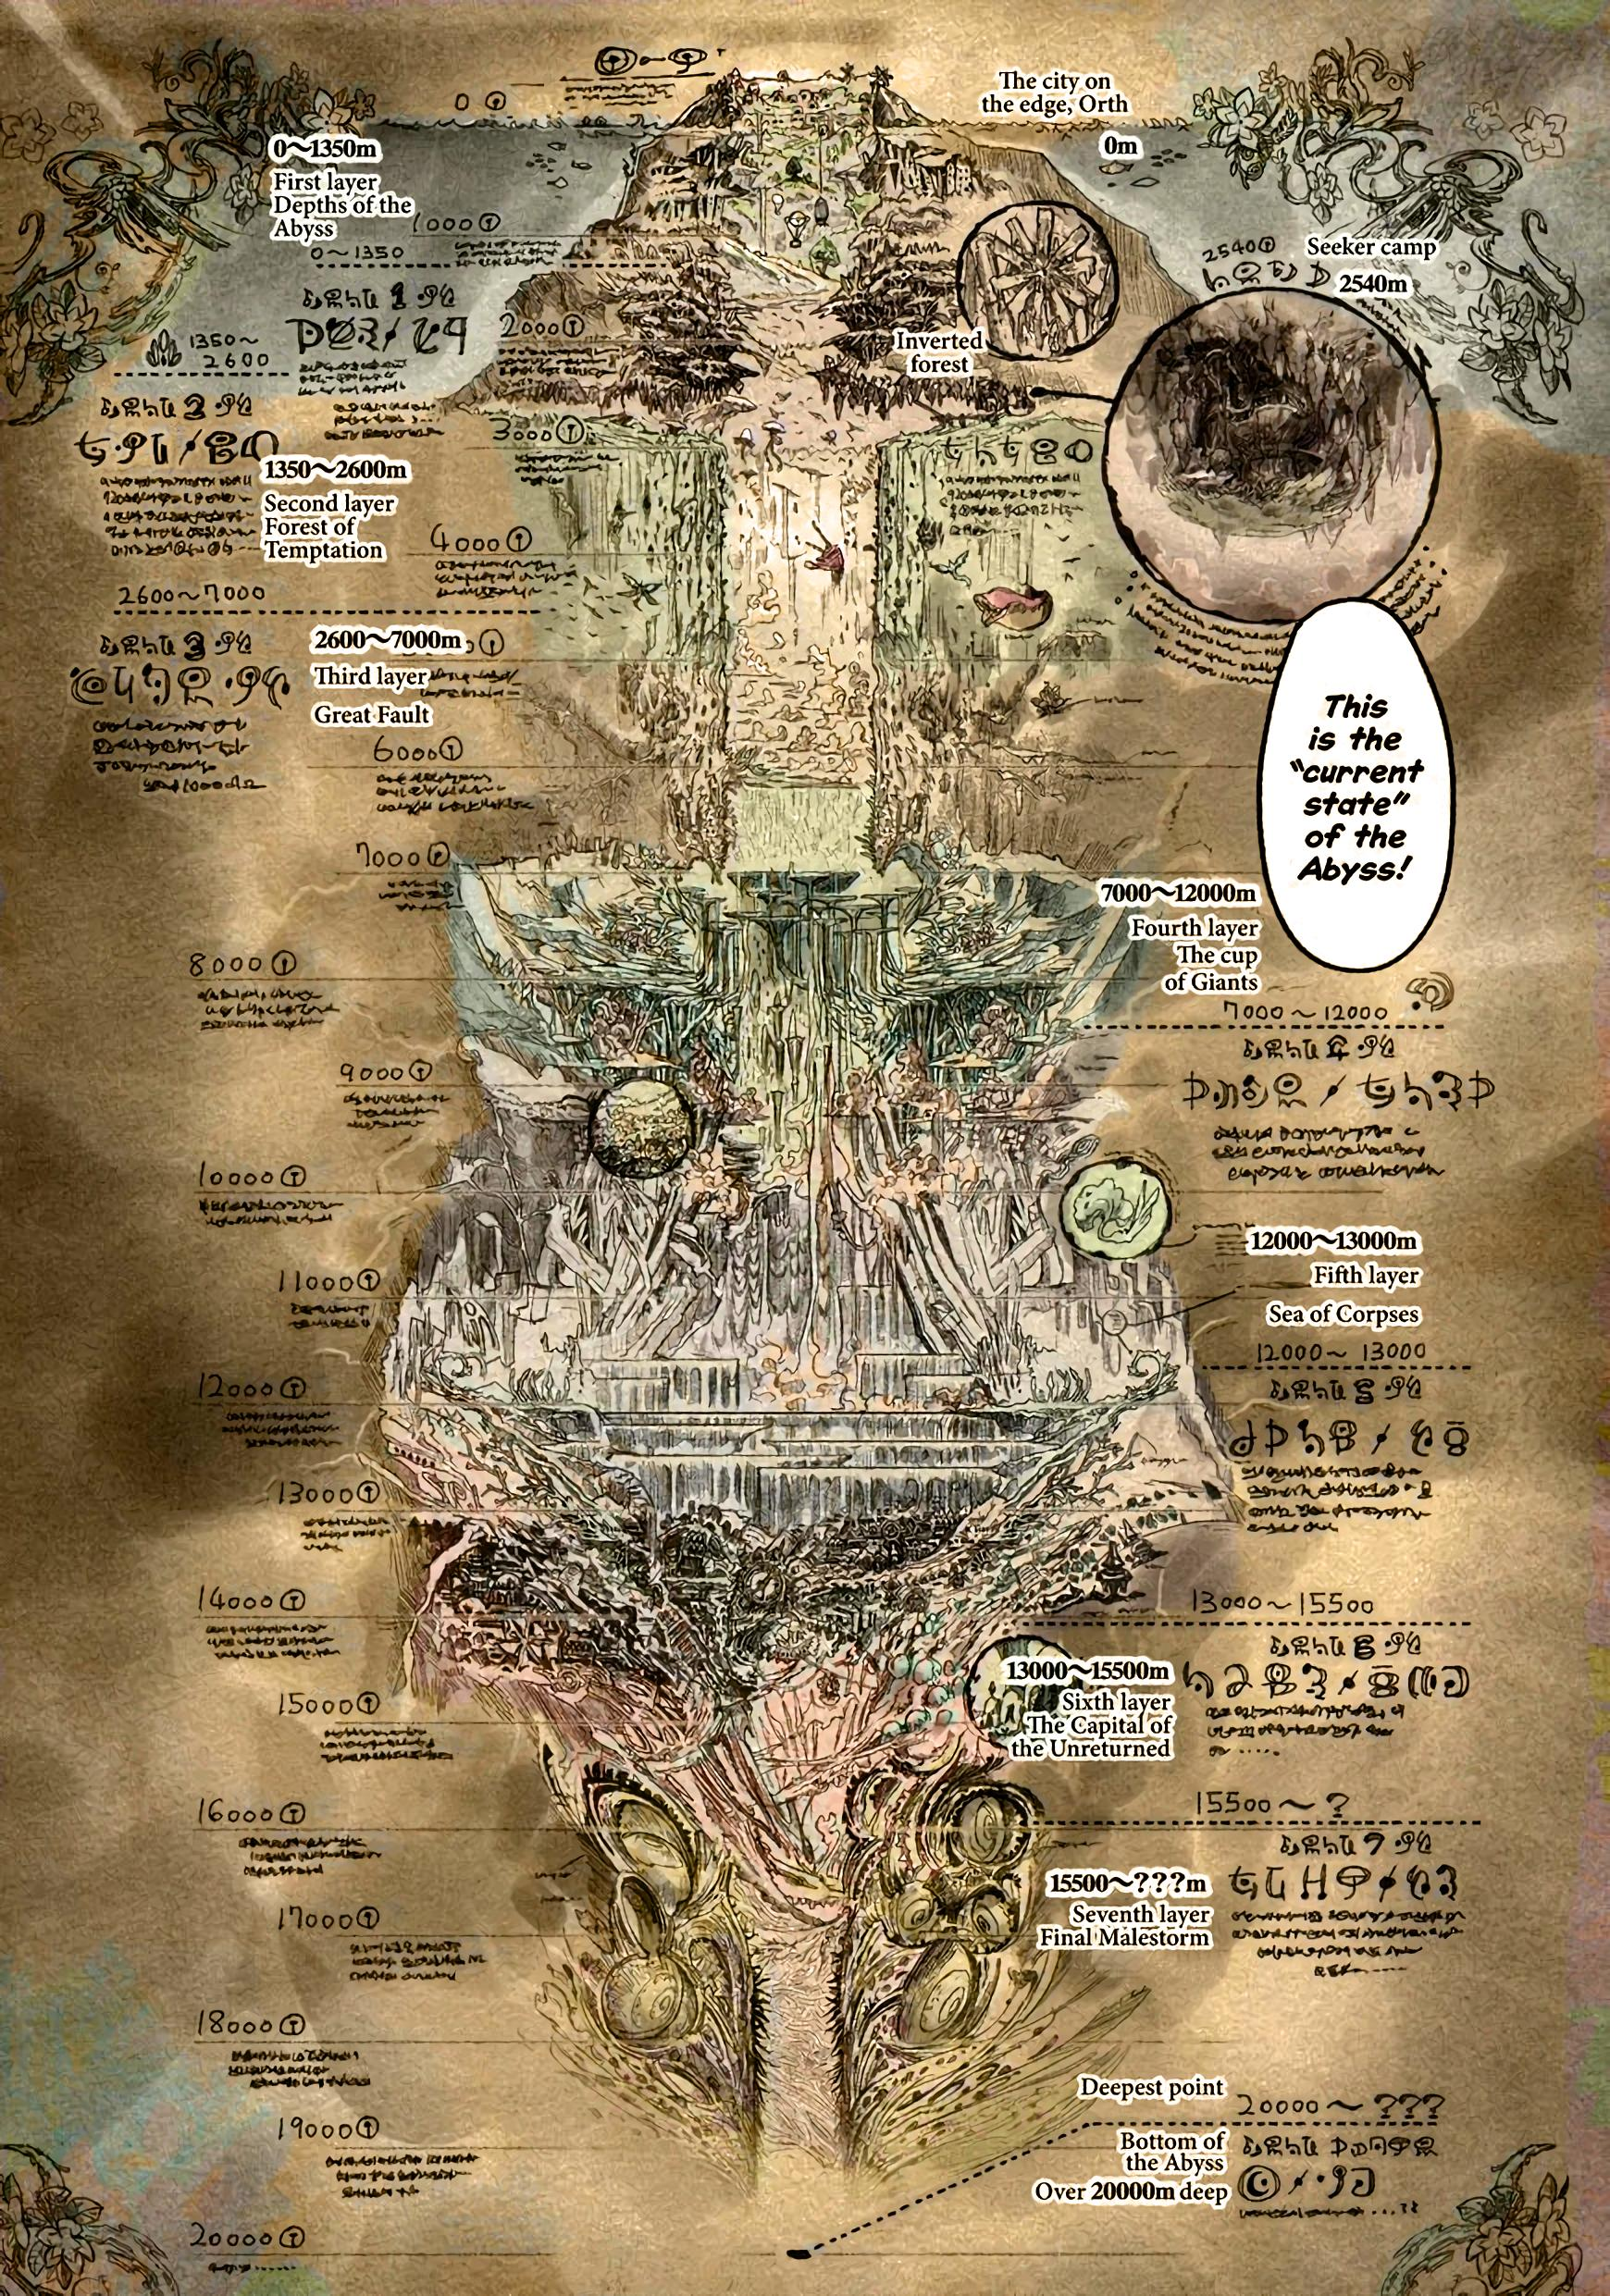
\includegraphics[width=\textwidth,height=.999\textheight]{img/descending/1506982818380.jpg}% Large image
    \clearpage
  }
  %\caption{Known map of the Abyss}
\end{figure}